%\chapter{Bayesian Neural Networks for Cancer Types Prediction}
%\chapter{Neuro-symbolic Representation Learning on Knowledge Graphs}
\chapter{Explaining with Decision Rules}\label{chapter:xai_rules}
\textit{``Compass rules direction; Decision rules life! ''}- Israelmore Ayivor

\section{Chapter Overview} \label{chapter_7:cw}
With the growing adoption of machine learning~(ML), there is a surge of research interest towards making ML models more transparent and interpretable~\cite{ming2018rulematrix}. In the previous chapters, how the \textit{multimodal convolutional autoencoder classifier}~(MCAE)-based models that were trained to extract most important features\footnote{Marker genes responsible for different types of cancer.} from the multimodal genomics data. By employing interpretable techniques, attempts were taken to mitigate the opaqueness of each `black-box' model.
Besides, different visualization plots were provided to explain the decisions. Explaining with plots or charts are mostly suitable for an ML expert, e.g., a data scientist as they are very helpful for exploration and debugging purposes. However, a large number of potential but neglected users are the domain experts~(e..g, medical doctors) with little to no knowledge of ML, but are expected to use the decision support system~(DSS) in a clinical setting~\cite{ming2018rulematrix}.

%In \cref{chapter:xai},  %We also provided explanations and interpretations of the learned knowledge\footnote{ \textbf{RQ4}: How to explain embedded domain knowledge, e.g.  mechanisms of carcinogenesis?}.

\hspace*{3.5mm} On the other hand, each MCAE model is a very complex deep neural network~(DNN) architecture trained on high dimensional multimodal genomics data. Due to highly non-linearity containing higher order interactions among features, those neural network-based models are very complex. Let's assume that $MCAE_{slr}$ and $MCAE_{lrc}$ models are now partially `white-box' models. Representing the learned knowledge in human understand-able form, e.g., as decision rules are more interpretable. A rule-based knowledge representation based on an interpretable model's input-output behavior can help understand, explore, and validate the embedded knowledge~\cite{ming2018rulematrix}. Since a rule only contains antecedents~(IF) and the consequent~(THEN), users can focus on understanding the learned knowledge itself without focusing much on the underlying latent representation of the data~\cite{ming2018rulematrix}. 

\hspace*{3.5mm} Decision rules are more effective at providing intuitive explanations. Using a set of rules, it is possible to explain a decision directly to humans with the ability to look up the reason for a decision. In this chapter, considering the limitations of plot-based explanations, model-agnostic explanations of the predictions are provided by based on the features extracted by MCAE-based models. Based on IF-THEN rules for the reasoning of a model's prediction are explained so that human users can understand.  %, which will be model-agnostic explanations based on IF-THEN rules. 
Representative rule sets for individual diagnosis cases are generated based on Scalable Bayesian Rule List~(SBRL) proposed by Yanget al.~\cite{BayesianRule}. The rule sets are then used to explain individual predictions of the black-box MCAE-based models w.r.t a surrogate model. 
This chapter hypothesize\footnote{\textbf{H8}: A surrogate model can be used to approximate the predictions~(embedded knowledge) of a partially `white-box' model and generate decision rules for diagnosis decisions.} that: i) a representative decision rule set generated by a surrogate model can sufficiently explains individual diagnosis decision~(i.e., prediction) of a partially white or black-box model, ii) a surrogate model can be used to approximate the predictions~(embedded knowledge) of a partially `white-box' model and generate decision rules for diagnosis decisions.
It is to note that the generated decision rules will be used for ontological reasoning in \cref{chapter:nsr} for generating fairer decision rules.

%Besides, tree-based approach is employed to explain the decisions both globally and locally and analyse potential wrong predictions. 

\section{Introduction} \label{chapter_7:intro}
DNNs are inherently opaque, making them difficult for users necessarily know which factor contributed to what aspect of the resulting score~\cite{ribeiro2018anchors}. Besides, due to the nested non-linear and complex structure, DNN architectures are mostly opaque and perceived as `black box' methods. They not only suffer from lack of transparency but also cannot reason about their underlying decisions. A DNN produces a prediction, which is an outcome of a bunch of mathematical expressions chained together that represent the way inner layers of an algorithm. Though the approaches based on DNN achieved a significant higher accuracy than linear models, in many healthcare problems, a simple logistic regression~(LR) model was thus chosen over DNN due to interpretability concerns. The reason is that domain experts felt that it was too risky to deploy the DNN-based model for decision making with patients because of such opaqueness. Though less accurate, LR fitted parameters have relatively clearer meanings, which can facilitate the discovery of problematic patterns in the dataset~\cite{ming2018rulematrix}. 

\hspace*{3.5mm} However, depending upon the requirements of the users and to understand the behavior of sophisticated ML models, interpretable ML techniques~(e.g., ranging from global to local explanations) have shown tremendous success that can be computed for any classifier. Even though, we have developed several models by embedding interpretability logic, whether humans understand a model enough to make accurate and trustworthy predictions about its behavior on unseen instances is a not clear~\cite{ribeiro2018anchors}. Local interpretability approaches mostly provide explanations to describe the local behavior of a model using a linearly weighted combination of input features~\cite{baehrens2010explain}. Although, linear functions can capture relative feature importance, whether they apply to an unseen instance is not clear, given that linear explanations are local. Besides, the coverage\footnote{Coverage w.r.t. rules signifies region where explanation applies.} is unclear, which can lead to low human precision~\cite{ribeiro2018anchors}. 

\hspace*{3.5mm} In the previous chapters, we have seen that explaining a diagnosis decision with plots and charts are good for exploration and discovery. We have seen how the models are helpful at predicting cancer types. However, interpreting them to patients may be difficult for the first time. For example, suppose the $MCAE_{lrc}$ model predicts that the selected patient has breast cancer in which model's average response~(i.e., intercept) on the GE+miRNA modality is +0.452. The model predicts that the selected patient was diagnosed with a probability of 75.3\%. It also displays all the variables that contributed to that prediction. Still, explaining them to a patient in a Lyman terms may be difficult unless they are explained in a simple human-interpretable way~(e.g., decision rule).  

\begin{figure}[h]
	\centering
		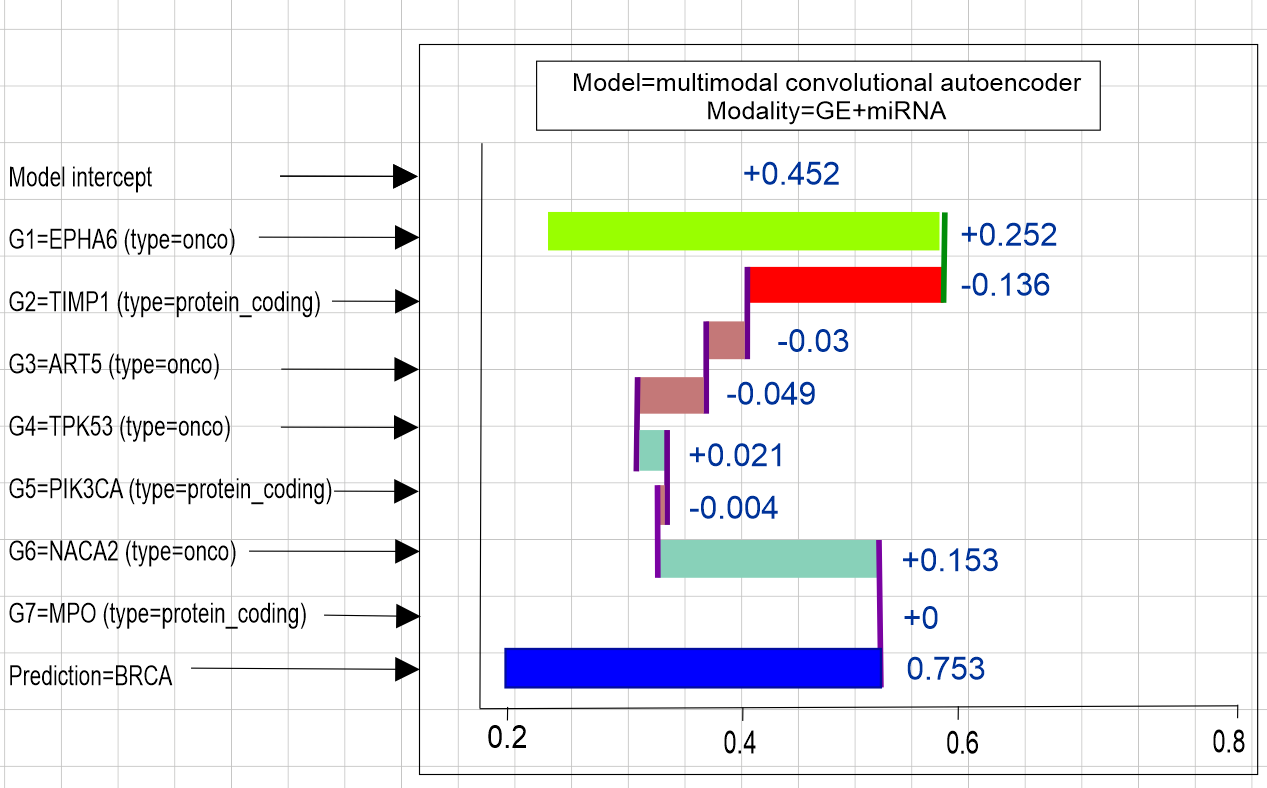
\includegraphics[scale=0.6]{images/intercept.png}
	    \caption{Explaining a diagnosis decision to patient is difficult unless it is interpreted simpler way}
	\label{problem_of_xai:1}
\end{figure}

\hspace*{3.5mm} Moreover, a doctor might want to understand the reasons behind any automatic diagnosis before making the final diagnosis decision. Domain experts may have knowledge that they learned in years of their research and clinical practice, which is what current ML models may fail to utilize~\cite{ming2018rulematrix}. 
%In this thesis, one of the goals is to generate human-interpretable decision rules automatically based on self-explanatory logic for all decisions. 
On the contrary, even this simple concept may not be well understood by the patient~\cite{post2015patient} themselves. However, once we have a transparent and easily explainable AI model, decision rules can be generated using a series of IF-THEN statements. Thus, using a set of rules, it possible to explain a decision intuitively to human with the ability to look up the reason for a decision. A decision rule is a simple \texttt{IF-THEN} statement consisting of a condition called antecedent and a conclusion~\cite{molnar2019interpretable}. The IF-THEN structure semantically resembles natural language and the way how human think~\cite{molnar2019interpretable}. 

\hspace*{3.5mm} Let's, consider a few exemplary samples and the model's prediction. Suppose we have a simple LR model for predicting the cancer types based on gene expression dataset. If the LR model made a prediction of certain cancer type and identified that patient gender, age, and a specific marker gene is contributing for this decision, then interpreting a predicted cancer type with a decision rule is very easy and can be explained in layman term. For example, \texttt{``IF you're female AND you're more than 50 years old AND top gene is TP53~(conditions), THEN you've breast cancer~(prediction)''}. Additionally, a doctor can provide further explanations\footnote{Based on his domain expertise.} saying that \textit{``an increased breast cancer is associated with risk for developing lymphedema, musculoskeletal symptoms, and osteoporosis"}. 

\begin{table}[h!]
    \caption{Exemplary samples and the model's prediction}
    \label{ge:rule_example}
    \vspace{-6mm}
    \begin{center}
        \scriptsize
        \begin{tabular}{l|l|l|l|l}
            \hline
            \rowcolor{Gray}
            \textbf{Sex} & \textbf{Age} & \textbf{Race} & \textbf{Gene} & \textbf{Cancer type} \\\hline    
            Female & 55 & American & TP53 & BRCA \\\hline
            Male & 49 & German & TBX3 & KIRC \\\hline
            Female & 68 & Canadian & TP53 & BRCA \\\hline
            Male & 72 & Egyptian & MPO & COAD \\\hline
        \end{tabular}
        \vspace{-6mm}
    \end{center}
\end{table}

\hspace*{3.5mm} Let's consider a complex example: \texttt{``IF sex = Female AND Age >= 50 AND gene = TP53 THEN PREDICT cancer type = BRCA''}. This example represents a representative rule set that can anchor LR model's underlying reasoning. Besides, the result also shows which attributes were taken into account by the model and it's patient sex, age, and biomarker. Such short and disjoint rules are easier to interpret than hierarchies like decision lists or trees~\cite{ming2018rulematrix}.
Thus, if derived from intelligible features and the length of the condition is short, decision rules are probably the most interpretable prediction models. Therefore, compared to other interpretable options, decision rules are trustable and easy to comprehend and understand than alternatives~\cite{ribeiro2018anchors}. 
%For instances where humans can confidently predict the behavior of a model, let(human) precision be the fraction in which they are correct(note that this is human precision, not model precision). High human precision is paramount for real interpretability - one can hardly say they understand a model if they consistently think they know what it will do, but are often mistaken. 
%Using rules~(and rules-based systems) to explicate machine learning results creates explainable AI. Many of the far-reaching applications of AI at the enterprise level — deploying it to combat financial crimes, to predict an individual’s immediate and long-term future in health care, for example — require explainable AI that’s fair, transparent and regulatory compliant. %Rules can explain machine learning results for these purposes and others.
%After organizations gain insight into the black box of intricate machine learning models, the best way to explain those results to customers, regulators and legal entities is to translate them into rules that, by their very definition, offer full transparency for explainable AI. Rules can also highlight points of bias in models.

\hspace*{3.5mm} The quality of a decision rule is measured in terms of support and accuracy. Support~(also known as coverage) of a rule is the percentage of samples to which the condition of a rule applies. Let's assume the surrogate or LR model generates a \texttt{``IF sex = Female AND gene = TP53 THEN PREDICT cancer type = BRCA''}. Suppose out of 5,000 cancer cases, patients of 200 cases are are aged above 50 years and TP53 is found to be the marker gene\footnote{The prediction or consequent~(THEN-part) is not important for the calculation of support.}, then the support of the rule is 4\%. 
The accuracy or confidence of a rule is a measure of how accurate the rule is at providing the correct diagnosis decisions~(i.e, the correct cancer type) for the samples to which the condition of the rule applies. Let's out of 200 beast cancer cases, where the \texttt{``sex = Female AND gene = TP53''} applies, 175 have \texttt{``cancer type = BRCA''}, 20 have \texttt{``cancer type = COAD''} and 5 have \texttt{``cancer type = KIRC''}, then the accuracy of the rule is 87.5\%. 
However, one know issue is the accuracy-support trade-off. Although, adding more features to the condition, may help improve the accuracy can be increased, but the support is reduces.

\hspace*{3.5mm} However, overlapping rules is a known challenge in rule based explanation~\cite{molnar2019interpretable}. Often rules can overlap. For example, imagine when we want to predict the cancer type of a sample, but two or more rules gives contradictory predictions. Consequently, the interpretability suffers when several such rules apply~\cite{molnar2019interpretable}. 

\begin{itemize}[noitemsep]
    \item \textbf{Overlapping rules} - rules can overlap. For example, imagine when we want to predict the cancer type of a sample, but two or more rules gives contradictory predictions. Consequently, the interpretability suffers when several such rules apply~\cite{molnar2019interpretable}. 
    \item \textbf{No single rule applies} - there is a possibility that even no single rule applies for an individual cancer case, except for the default decision rule.  
\end{itemize}

\hspace*{3.5mm} To overcome this, a decision list or a rule set can be created by combining most influential rules. In other words, decision lists and decision sets are two main strategies for combining multiple rules. 
%The former represent a representative ordered rule list, the latter an unordered rule list. %: Decision lists (ordered) and decision sets (unordered). Both strategies imply different solutions to the problem of overlapping rules.
A decision list signifies the order to the decision rules~\cite{molnar2019interpretable}. If the condition of the first rule is true, the diagnosis prediction of a DSS can be generated on the first rule. Otherwise, it is reasonable to continue checking next and subsequent rules, and so on. This way, decision lists can solve the problem of overlapping rules by returning the prediction of the first rule only~\cite{molnar2019interpretable}. On the other hand, a decision set resembles a representativeness of the rules, except that some rules might have a higher voting power~\cite{molnar2019interpretable}. 
%According to set theory, rules are either mutually exclusive, or there is a strategy to resolve the conflicting rules. One of the techniques is ranking rules based on weighted majority voting of individual rule accuracies~\cite{molnar2019interpretable}. 

\hspace*{3.5mm} Although, the issue of overlapping rules can be solved using decision lists and sets, they can still suffer from another potential issue known as ``no rule applies''. Sometimes there is a possibility that even no single rule applies for an individual cancer case.
This issue can be resolved by introducing a default rule. The default rule applies when no other rule applies for specific samples~\cite{molnar2019interpretable}. The prediction of the default rule is often the majority class of the data points that are not covered by other rules in the decision list or rule sets~\cite{molnar2019interpretable}. An exhaustive set or list of rules can be generated by covering the entire feature space. 
%By adding a default rule, a set or list automatically becomes exhaustive.

\hspace*{3.5mm} In this chapter, model-agnostic explanations of the predictions are provided by based on the features extracted by MCAE-based models. In particular, based on IF-THEN rules for the reasoning of a model's prediction are explained so that human users can understand. Further, the generated decision rules will be utilized for ontological reasoning to generate fairer decision rules in \cref{chapter:nsr}. Overall, the goal of this chapter is to answer the following sub-questions for RQ3\footnote{\textbf{RQ3}: \textit{How to provide human-understandable interpretations of the decisions using decision rules?}}: 

\begin{enumerate}[noitemsep]
    \item What rules did the model learn?
    \item What variables did the model use to make the predictions?
    \item What representative rules that can be considered descriptive for the Oracle model?
    \item What are the behaviors of the model that the surrogate is not able to approximate~(i.e., simulate)?
    \item Can we reuse the rules to validate the findings to mitigate decision biases? 
\end{enumerate}

\hspace*{3.5mm} The rest of the chapter is structured as follows: \cref{chapter_7:rw} covers some related works on interpretable decision rules and summarize their potential limitations. \Cref{chapter_7:mm} describes the approach of generating explainable decision rules. \Cref{chapter_7:results} demonstrates some evaluation results and discusses key findings of the study. \Cref{chapter_7:conclusion} provides some explanations of the importance and relevance of the study reported, highlights the limitations and discuss some future works before concluding the chapter.  

\section{Related Work} \label{chapter_7:rw}
A number of approaches that have been proposed construct globally interpretable models. With such models, the user should be able to guess the model’s behavior on any example - perfect coverage. However, these models are not appropriate for many domains, e.g., almost no interpretable rule-based system is suitable for text or image applications, due to the sheer size of the feature space, or are just not accurate enough. However, since interpretability comes at the cost of flexibility, accuracy, or efficiency, an alternative is learning a simple interpretable model to imitate the black-box model globally. For example, a decision tree or a set of rules can yield low human precision~\cite{molnar2019interpretable}. Simple models are not able to fully capture the behavior of the complex ones, and thus lead users to wrong conclusions, especially since it is not clear when the simple model is faithful~\cite{bhatt2020explainable}. 

\hspace*{3.5mm} To avoid this issue, local model-agnostic explanations can be used to explain individual predictions, instead of explaining the whole model at once or globally. For example, Local Interpretable Model-agnostic Explanations~(LIME)~\cite{LIME}. While the complex logic underlying the whole model may be too much for a surrogate model to learn, the logic for one instance or a group of similar instances\footnote{For example, co-expressed genes in a patient's genomic profile} may be simple enough. LIME was used to better understand why some patients were misclassified by a black-box model predicting survival after cardiac arrest. However, a LIME model for a patient that was mis-predicted to survive showed that the black box model was too heavily influenced by certain features, e.g. healthy. 

\hspace*{3.5mm} These methods provide a trade-off: each explanation is easy to understand even for complex models and tasks, but only captures the behavior of the model on a local region of the in-put space. Together with many forms of linear explanations, anchor-based approaches have been used to explain the reasoning for complex models for use cases such as machine translation and video question answering system. Rule-based models are composed of logical representations, i.e., \texttt{``IF-THEN-ELSE''} statements pervasively used in programming languages. Typical representations of rule-based models include decision tables, decision trees, and rule sets or decision lists~\cite{BayesianRule}. Trees are hierarchical data structure that have been widely. BaobabView uses a node-link data flow diagram to visualize the logic of decision trees, which inspired our design of data flow visualization in rule lists~\cite{ming2018rulematrix}. 

%In a later position paper, Freitas et al. summarized a few good properties rules and tables possess that trees do not. Previous studies used pure texts to present rules.  %In our study, we provide a graphical representation of rule lists as an alternative for navigating and exploring proxy models.

\hspace*{3.5mm} To deal with overlapping and contradictory rules, OneR~(aka. learn rules from a single feature), sequential covering, and Bayesian rule lists are three widely proposed approaches to learn rules from the training data. Holte et al.~\cite{holte1993very} proposed OneR, which learns rules from a single feature, where a most representative or influential rule from the entire feature space is selected~\cite{molnar2019interpretable}. Sequential covering is a general procedure that iteratively learns a single rule to create a decision list or set that covers the entire training dataset rule-by-rule, by removing the data points that are already covered by the new rule~\cite{molnar2019interpretable}. On the other hand, Bayesian rule lists combine pre-mined frequent patterns into a decision list using Bayesian statistics~\cite{molnar2019interpretable}.
Although surrogate model-based explanations and the rules are found easy for human interpretability, due to highly non-linearity containing higher order interactions among features in very complex DNN model. Consequently, an interpretable surrogate model may not learn such complex interactions. To overcome this, one approach is to generate a surrogate model trained on the simplified data containing most important features~\cite{molnar2019interpretable}.
%Due to highly non-linearity containing higher order interactions among features, surrogate models is that black box models based on DNNs are often highly complex. This is a major reason why an interpretable surrogate model may not learn such complex interactions. To overcome this, one approach is to generate a surrogate model trained on the simplified data containing most important features.

\hspace*{3.5mm} Recently, the neural-backed decision tree~(NBDT) is proposed by ~\cite{wan2020nbdt}. Unlike regular DNN architectures, NBDT can output intermediate decisions for a prediction. For example, given an image, NBDT can output both Dog and Animal, Chordate, Carnivore, etc. as a sequence of decision rules, while a neural network may output only Dog. DBDT constructs an induced hierarchy for the decision tree. This hierarchy yields a particular loss function, which we call the Tree Supervision Loss. DBDT starts the inferencing by passing the sample through the DNN backbone before the final fully-connected softmax layer. Then the inference is finished by running the final fully-connected softmax layer as a sequence of decision rules, which they called embedded decision rules. These decisions are subsequently culminated in the final prediction by preserving high-level interpretability. 

\hspace*{3.5mm} Unfortunately, these approaches put less focus on how visualization can help analyze decision tables and rule lists. In particular, apart from tree-based decision rule visualization, research communities put less focus on handling very long deciison list and filtering from user-friendly interface for non-technical experts. Nevertheless, the lack of interest in visualizing decision tables and rule lists is partially due to the fact that they are not naturally graphical representations as trees~\cite{ming2018rulematrix}. There is also no consensus that trees are the best visual representations for understanding rule-based models~\cite{ming2018rulematrix}. Huysmanset al.~\cite{mehrabi2019survey} has showed that decision tables are the most effective representations, while other studies disagrees.

\section{Methods} \label{chapter_7:mm}
In this section, we discuss our approach in detail, including data collection, preprocessing, network construction, and training, followed by interpreting the network towards biomarkers identification. 

\subsection{Problem statement}
%To explain a model's local and global behaviours, 
The problem is to generate a set of rules capable of ``anchoring"~(covering) the prediction sufficiently, by approximating entire model's behaviour. Since it is already argued that the interpretability provided by the predictor ${f}$ in \cref{chapter:xai} is not sufficiently human-interpretable and globally too complex, it would not be fair to claim ${f}$ a fully `white-box' model. For a given model\footnote{For the simplicity, it would be reasonable to assume ${f}$ is  still a `black-box' model, albeit it is `white-box' to a major extent.} ${f}: X \rightarrow Y$, the goal of local model-agnostic interpretability is to explain individual predictions ${f}(x)$ for an instance~(i.e., $x \in X$) using decision rules, where $X$ are the training samples\footnote{Top 660 features generated by both $MCAE_{lrc}$ and $MCAE_{slr}$ on the text set in \cref{chapter:xai} forms the feature space.} and $Y$ are provided ground truths. %, where $X$ is the full dataset and ${F}(x)$ is the individual prediction for $x$. 

\begin{table}[h!]
    \caption{Example of gene expression samples based on oncogenes}
    \label{ge:ancor_example}
    \vspace{-6mm}
    \begin{center}
        \scriptsize
        \begin{tabular}{l|l|l|l|l|l|l|l|l|l}
            \hline
            \rowcolor{Gray}
            \textbf{Type} & \textbf{Gender} & \textbf{Age} & \textbf{Race} & \textbf{TP53} & \textbf{TBX3} & \textbf{MTOR} & \textbf{MPO}  & .. & \textbf{AMBN} \\\hline    
            BRCA~(1) & 1 & 55 & American & 0.3195 & -0.2154 & -0.154 & 0.4767  & .. & 0.652 \\\hline
            BRCA~(1) & 1 & 49 & Bangladeshi & 0.230 &  -0.552  & 0.715  & 0.924   & .. & 0.552 \\\hline
            BRCA~(0) & 0 & 68 & Canadian & -0.240 &  0.252  & 0.350  & -0.642  & .. & -0.985 \\\hline
            BRCA~(0) & 0 & 72 & Egyptian & -0.450 &  0.012  & 0.650  & -0.325  & .. & 0.357 \\\hline
        \end{tabular}
        \vspace{-4mm}
    \end{center}
\end{table}

%\hspace*{3.5mm} Providing human-level interpretability by "zooming in" on individual predictions makes the explanation task easier and trustworthy\cite{ribeiro2018anchors}. %Nevertheless, since both perturbations $\mathcal{D}$ and explanations must use an interpretable representation even if the model uses an alternative representation of the input, we employed a model-agnostic method called anchor\cite{ribeiro2018anchors}, which works by perturbing the instance $x$ according to some ``perturbation distribution" $\mathcal{D}$.  

\begin{sidewaysfigure*}
	\centering
		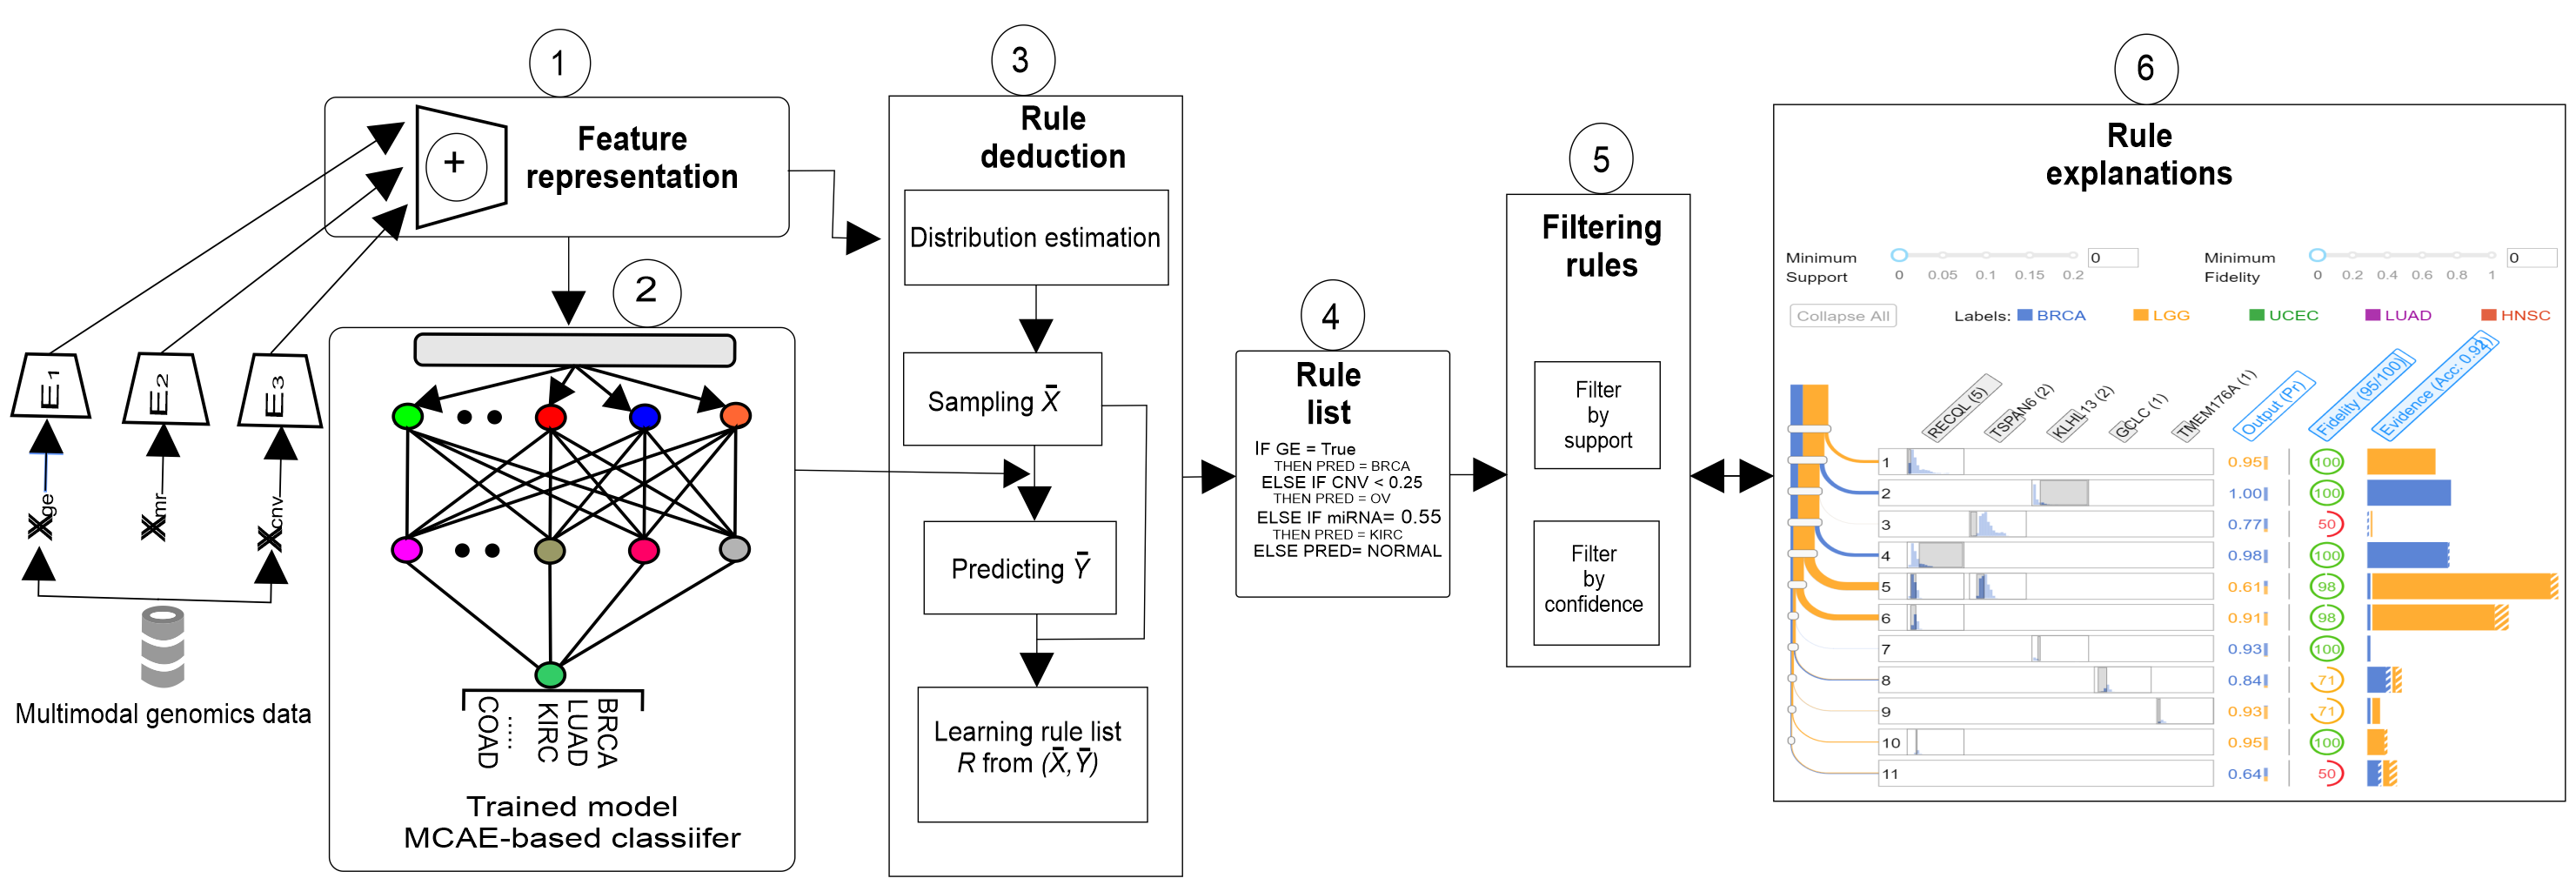
\includegraphics[scale=0.7]{images/rules_wf.png}
	    \caption[The rule generation and explanation workflow]{The rule generation and explanation workflow: (1) multimodal genomics data is used to create for learning\\ representation, (2) a model is trained, (3) model produces a rule list by approximating it's behaviour, (4) rule\\ list is filtered based on given support and confidence, before (5) explaining the decision} 
	    \label{fig:rules_wf}
\end{sidewaysfigure*}

\hspace*{3.5mm} Let $R$ be a rule~(in the form of set of predicates) to provide interpretable representation, such that $R(x)$ returns 1 if all its feature predicates are true for instance $x$, 0 otherwise. For example, in \cref{ge:ancor_example} when x=\{1, 0.3195, -0.2154, -0.154, 0.4767, 0.652\} or x=\{1, 0.230, -0.552, 0.715, 0.924, 0.652\}, $f(x)=Y$, $A(x)=1$ where $A=\{TP53, TBX3, MPO, AMBN\}$. On the other hand, when x=\{0, -0.240, 0.252, 0.350, -0.642, -0.985\} or x=\{0, -0.450, 0.012, 0.650, -0.325, -0.357\}, $f(x)=N$, $R(x)=0$ where $R=\{TP53, TBX3, MTOR, MPO\}$. Representing a decision this intuitive way is not very user friendly given the continuous nature of the data and huge number of feature space. Therefore, we need a better rule list to approximate the behaviour of the original models trained on dataset $X$. 

\subsection{Generating decision rules}
First, the MCAE model is trained on multimodal genomics data to learn the latent representation. Global attention mechanism is then applied on the learned representation to disentangle and most important variables or cancer marker genes~(i.e., 660 marker genes). A surrogate model is subsequently trained on the identified features to produce a rule list by approximating the behaviour of the  models. Then Bayesian rule-based approach called \texttt{Scalable Bayesian Rule List}~(SBRL) is employed to solve the overlapping decision rules and generate decision set. The decision sets are subsequently used to explain the surrogate model's decision. The overall workflow of the rule generation is shown in \cref{fig:rules_wf}.

\hspace*{3.5mm} Since not all the rule may not qualify w.r.t. coverage, support, and confidence, a filtering option is added for the users. Support and confidence are the two thresholds that can be set to get the filtered rules, before explaining the final decision to the patients. Since, representation learning and predictive modelling are already covered, only the decision tree and tree ensemble based model surrogation, rule generation, filtering of rules, and rule-based explanation steps are covered in the subsequent sections. 

\subsubsection{Model surrogation}
A surrogate model is an interpretable model trained to approximate the underlying model as closely and accurately as possible. By interpreting the surrogate model, we can draw conclusions about the `black box' model~\cite{molnar2019interpretable}. The goal here is to approximate the `black-box' prediction function $f$ with the surrogate model prediction function $g$, under the constraint that $g$ is interpretable. Since any interpretable model can be used for function $g$~\cite{molnar2019interpretable}, a decision tree-based gradient boosted trees~(GBT) classifier is trained. That is, gradient boosting is performed on the base estimator~(i.e., decision trees). 

\hspace*{3.5mm} A decision tree is a simple tree structure that iteratively splits the data multiple times w.r.t to threshold values of the features. At each node of the tree, the dataset is splitted into multiple subsets until each subset contains instances from one class only~(With the hope that the leaf node in the tree is pure). Starting from the root node, the next nodes are checked by tracing the path down to the leaf, which forms a rule. In a decision tree, the relationship between a predicted label $\hat{y}$ and a feature $x$ is defined as~\cite{di2019surrogate}: 

\vspace{-2mm}
\begin{align}
    \hat{y}_{i}=\hat{f}\left(x_{i}\right)=\sum_{j=1}^{N} c_{j} I\left\{x_{i} \in R_{j}\right\},
\end{align}

\hspace*{3.5mm} where each sample $x_{i}$ reaches exactly one leaf node, which can be described as a subset $R_{j}$ of the dataset. The identity function $I\{.\}$ represent the combination of rules at each of the internal nodes~\cite{di2019surrogate}.

During the boosting phase, the splitting criteria used at every level of the tree is considered a pair $p=(k, v)$ w.r.t features such that $k=$ $1,2,3,4,5 \ldots, m$ with threshold value $v \in R$. The splitting divides the criteria feature vector $X$ into following two disjoint subsets of $X^{L}$ and $X^{R}$, for each $x=\left(x^{1}, \ldots, x^{m}\right) \in X$~\cite{al2021cdrgi}:

\vspace{-4mm}
\begin{align}
    X=\left\{\begin{array}{lll}X^{L} & \text { if } & x^{k} \leq V \\ X^{R} & \text { if } & x^{k} \geq V\end{array}\right.,
\end{align}

\hspace*{3.5mm} where the splitting criteria is defined as $\operatorname{argmin}\{P(r, f, M) \}$ in which $M$ calculates the optimality of both splitting rule $r$ and collection $M$ w.r.t target function $f, P$ as follows~\cite{al2021cdrgi}: 

\vspace{-2mm}
\begin{align}
    P(r, f, M)=\frac{1}{\sum_{i=1}^{s}\left|X_{(i)}\right|}\left(\sum_{i=1}^{s}\left|X_{(i)}^{L}\right| \operatorname{Var}\left(f\left(X_{(i)}^{L}\right)\right)+\left|X_{(i)}^{R}\right| \operatorname{Var}\left(f\left(X_{(i)}^{R}\right)\right)\right),
\end{align}

\hspace*{3.5mm} where $f\left(X_{(i)}\right)$ is the score of target samples $X_{(i)}$.  However, interpreting a long rule set containing a large number of antecedents and containing continuous values in involved, is very difficult. Therefore, RuleMatrix uses the minimum description length binning~(MDLB)\footnote{\url{https://github.com/hlin117/mdlp-discretization}} discretization to discretize the features and the frequent mining algorithm called \texttt{FP-growth}~\cite{han2000mining} to get the candidate rule sets based on which the final rule set is generated. However, in our case, MDLB was not a feasible option to employ, due to continuous feature space in the training dataset. 

\hspace*{3.5mm} Maslove et al.~\cite{maslove2013discretization} has shown that discretization helps not only to get better accuracy, but also at interpreting  decision rules better. This requires the input features to be categorical, while our dataset has a continuous feature space. Therefore, we come up with our own discretization based on domain knowledge. There are many ways to cut a continuous feature into intervals, but this is not trivially straightforward way. This evolves an important consideration on number of intervals the feature should be divided into. Employing two splitting criteria such as quantiles and fixed interval lengths could be an option. For the former, one can binning continuous features based on the frequency of the values by quantiles is an option. However, it could end up with so many bins that would not help in interpreting a rule in human understandable way. 
%Although genomics data used are also mostly continuous, domain expertise or knowledge might help. 
According to baseline expression results, both gene expression and miRNA expressions are discritized into 4 different levels\footnote{\url{https://www.ebi.ac.uk/gxa/FAQ.html}}:

\vspace{-2mm}
\begin{itemize}[noitemsep]
    \item \textbf{Below} - if expression level is less than the cutoff~(0.5 FPKM\footnote{FPKM: Fragments Per Kilobase Million- is a normalised estimation of gene expression based on RNA-seq data.}).
    \item \textbf{Low} - if expression level is between 0.5 to 10 FPKM.
    \item \textbf{Medium} - if expression level is between 11 to 1000 FPKM. 
    \item \textbf{High} - if expression level is higher than 1000 FPKM. 
\end{itemize}

\hspace*{3.5mm} In many cases, CNVs can encompass genes leading to imbalances, e.g., genes that were thought to always occur in 2 copies per genome have now been found in 1, 3, or more than 3  copies\footnote{\url{https://www.gene-quantification.de/cnv.html}}. This findings also reflected in our data. Based on this assumption, we use the segmentation mean as the basis for computing the change in numeric values and discritized CNV features into 3 different levels:  

\vspace{-2mm}
\begin{itemize}[noitemsep]
    \item \textbf{Normal} - if CNV has exactly 2 copies.
    \item\textbf{Low} - if CNV has a low number of copy\footnote{Due to copy number deletion} ranging [-4, 1], i.e., less than normal copies.
    \item\textbf{High} - if CNV has a high number of copy\footnote{Due to copy number gain, but in some rare cases, number of copy is greater than 4.} ranging [3 and 4].  % than normal copy~(i.e., 2).
\end{itemize}
\vspace{-2mm}

\hspace*{3.5mm} Training a surrogate model is a model-agnostic method as it does not require knowing inner working principle of the `black-box' model. Since important features are already identified with the MCAE models, training a surrogate model is trivial. Technically, a student model is necessarily a `surrogate model' - a simplified version of the teacher model, which maps $Y_\text{sample}=f(X_\text{sample})$ to approximate the original model $f$~\cite{forrester2008engineering}. In the context of Bayesian statistics, we want to optimize a function $Y=f(x)$, which is very expensive to evaluate. Instead, we one optimize the surrogate model $Y_\text{sample}=f(X_\text{sample})$, which is faster to evaluate and we assume will reasonably represent the original model's behaviour. 

\hspace*{3.5mm} We create sample ${X}_{\text {sample}}$ based on the original model $f$ predicts the labels, where the number of samples is a customizable parameter set by human, e.g., data scientist. Subsequently, the sampled data ${X}_{\text {sample}}$ and the labels ${Y}_{\text {sample}}$ are used to generate the rule list. Overall, this is an optimization problem, where the objective is to maximize the fidelity of the rule list~\cite{ming2018rulematrix}.  
%We measured the performance of the surrogate model itself using $R^2$ to measure how well the surrogate replicates the `black-box' model.    

\vspace{-6mm}
\begin{align}
    \text {fidelity}(R)_{{X}}=\frac{1}{|{X}|} \sum_{\boldsymbol{x} \in {X}}[f(\boldsymbol{x})=R(\boldsymbol{x})],
    \label{eq:fidelity}
\end{align}

\hspace*{3.5mm} where $f(\boldsymbol{x})=R(\boldsymbol{x})$ is 1 if $f(\boldsymbol{x})=R(\boldsymbol{x})$, 0 otherwise. If the underlying ML model is to be replaced with another, the surrogate model will still be usable~\cite{molnar2019interpretable}. 

%\vspace{-2mm}
\begin{algorithm*}[h]
\caption{Generating surrogate model}
\small{
    \DontPrintSemicolon \SetKwInOut{Input}{Input}%
    \SetKwInOut{Output}{Output}%
    \Input{Dataset $X$ for training the `black-box' model $M_b$ or a new dataset from the same distribution for training the surrogate model, interpretable model type $t$ and params $p$.}%
    \Output{A surrogate model $M_s$ and predictions $Y_s$ to approximate `black-box' model $M_b$.}%
    \BlankLine%
    \For{for each sample $x \in X$}{\tcp*{For dataset $X$, get  predictions for black box model $M_b$}
        \vspace{-2mm}
        $Y_b \leftarrow  M_b.predict(X)$\;
        \textbf{Return} $Y_b$  
    }
    \BlankLine%
    \For{for each sample $x \in X$}{\tcp*{for each sample in training set do}
        \vspace{-2mm}
        $M_s \leftarrow  \{\}$\;
        $Y_s \leftarrow  \{\}$\;
        $t \leftarrow  \{\}$\; \tcp*{e.g., linear model, decision tree}
        %\vspace{-2mm}
        $clf \leftarrow  estimatorInstantiate(t,p)$\;\tcp*{Instantiate an interpretable estimator}
        \vspace{-2mm}
        $M_s \leftarrow  clf.fit(X, Y)$\; \tcp*{train the interpretable model $M_s$ on dataset $X$}
        \vspace{-2mm}
        $Y_s \leftarrow  M_s.predict(X)$\; \tcp*{Get the predictions of the surrogate model}
        \textbf{Return} $[(M_b, Y_b)(M_s, Y_s)]$
     }}
     \label{algo:surrogate_model_generation}
\end{algorithm*}

\hspace*{3.5mm} \Cref{algo:surrogate_model_generation} outlines the steps to obtain a surrogate model. Once a surrogate model is trained, R-squared measure~($R^2$) is calculated to measure how well the surrogate model replicates the `black-box' MCAE model~\cite{molnar2019interpretable}. The $R^2$ can be measured mathematically, as follows~\cite{molnar2019interpretable}: 

\begin{equation}
    R^{2}=1-\frac{SSE}{SST}=1-\frac{\sum_{i=1}^{n}\left(\hat{y}_{*}^{(i)}-\hat{y}^{(i)}\right)^{2}}{\sum_{i=1}^{n}\left(\hat{y}^{(i)}-\overline{\hat{y}}\right)^{2}},
    \label{ew:r_squared}
\end{equation}

\hspace*{3.5mm} where $\hat{y}_{*}^{(i)}$ is the prediction for the $i^{th}$ instance of the surrogate model $M_s$, $\hat{y}^{(i)}$ is the prediction of the `black-box' model $M_b$, $\overline{\hat{y}}$ the mean of the `black-box' model predictions, $SSE$ is the sum of squares error, and $SST$ is the sum of squares total~\cite{molnar2019interpretable}. The $R^2$ can be interpreted as the percentage of variance captured by the surrogate model will be used to explain the diagnosis decision, as follows~\cite{molnar2019interpretable}:

\begin{itemize}[noitemsep]
    \item If $R^2$ is close to $1(=$ low $\mathrm{SSE}$), then the surrogate model approximates the behavior of the `black-box' model very well. Subsequently, the complex model can be replaced with the surrogate model. 
    \item If $R^2$ is close to 0~(i.e., high SSE), the interpretable model will fail to explain the `black-box' model. In such scenario, we should not replace  complex model with the interpretable model.
\end{itemize}

\subsubsection{Rule set generation}
For a given surrogate model ${f}$, the task is to extract a rule list $R$ to explain it's decision. However, each modality in the multimodal genomic dataset has a large number of features. RuleMatrix~\cite{ming2018rulematrix} that was proposed for binary classification problem is extended for multiclass classification problem. In other words, the output distribution of RuleMatrix is extended to multinomial instead of binomial. 
As shown in \cref{fig:rules_wf}, we treat the original~(trained) model as a teacher that have sufficient knowledge and the student model is trained using the data ``labeled" by the teacher, s.t. the predictions of the teacher model is used as ground truth instead of the real ones. Nevertheless, since we have access to both a trained model and the data used to train the model, estimating the distribution of the training data ${X}$ is feasible. 

%\vspace{-2mm}
\begin{algorithm*}[h]
\caption{Initial decision list generation based on Scalable Bayesian Rule List}
\small{
    \DontPrintSemicolon \SetKwInOut{Input}{Input}%
    \SetKwInOut{Output}{Output}%
    \Input{Trained surrogate model $M_b$ and the list of default rules $D$}%
    \Output{Initial decision list in~(rule, probability) pairs}%
    \BlankLine%
    \textbf{Step-1}: generate the list of pre-mined frequent patterns from FP-Growth trees $F$.\;
    \textbf{Step-2}: Sample the list length parameter $m$ from a truncated Poisson distribution.\;
    \textbf{Step-3}: \For{for each default rule $d \in D$}{\;
        \vspace{-2mm}
        $\Tilde{D} \leftarrow$ Sample the Dirichlet-multinomial distribution parameter $\theta_0$ for target cancer type.\;
        \textbf{Return} $\Tilde{D}$  
    }
    \textbf{Step-4}: \For{Decision list rule $\mathrm{j}=1, \ldots, \mathrm{m}, \mathrm{d}$ 0}{\;
        \vspace{-2mm}
        Sample the rule length parameter $I$ number of conditions for rule $j$.\;
        Sample a condition of length $l_{j}$ from the pre-mined conditions $F$.\;
        $\Tilde{D_t} \leftarrow$ Sample the Dirichlet-multinomial distribution parameter for the antecedents.\;
        \textbf{Return} $\Tilde{D_t}$  
    }
    \BlankLine%
    \textbf{Step-5}: \For{For each sample in the dataset $x \in X$}{\;
        \vspace{-2mm}
        $R \leftarrow \{\}$\;
        $r \leftarrow$ Find the rule from the decision list $\Tilde{D_t}$ that occurs first.\;
        $p \leftarrow$ Draw the predicted outcome from the binomial probability distribution for rule $r$.\;
        $R \leftarrow r \cup p$\;
        \textbf{Return} $R$  
        }
    }
    \label{algo:initial_decision_lis_generation}
\end{algorithm*}

\hspace*{3.5mm} Unlike RuleMatrix, this approach does not require the joint distribution estimation~(i.e., for discrete and continuous features), given that our feature space is continuous. RuleMatrix takes a trained model~(i.e, teacher) and training\footnote{The number of driver genes identified the teacher model} set as input to produce a decision list or rule set.
Besides, the objective is to approximate the teacher model's behaviour via the surrogate model w.r.t, fidelity as the accuracy. On the other hand, since the surrogate model can reach it's decision through multiple rules with excessive length and  
%applying sequential covering\footnote{A procedure that repeatedly learns a single rule to create a decision list~\cite{molnar2019interpretable}} the entire dataset rule by rule was not what we optimally think. 
considering the length of number of predictors~(i.e, features), we apply the representation of an ordered list of inclusive rules based on SBRL. 

\hspace*{3.5mm} \Cref{algo:initial_decision_lis_generation} shows the pseudocode for the generation of an initial decision list generation based on SBRL. In SBRL, pre-mined frequent patterns are combined into a decision list using Bayesian statistics~\cite{molnar2019interpretable}, where the frequency of a pattern is measured in terms of its support in the entire training dataset~\cite{molnar2019interpretable}:

\vspace{-6mm}
\begin{align}
    \begin{array}{cl}
        \text {Support}\left(x_{j}=a\right)=\frac{1}{n} \sum_{i=1}^{n} I\left(x_{j}^{(i)}=a\right) \\
         \text {s.t.} & I \in[0,1],
    \end{array}
    \label{eq:support_eq}
\end{align}

\hspace*{3.5mm} where $a$ or $x_j$ is the feature value for $i$th sample, $n$ the number of data points in the dataset and $I$ the indicator function that returns $1$ if the feature $x_{j}$ of the instance $i$ has level $a$, otherwise $0$. 

\subsubsection{Filtering rules}
%In contrast, even though LIME uses the same $\mathcal{D}$, anchors adapt their coverage to the model's behavior and makes their boundaries clear. 
% Anchors are intuitive, easy to comprehend, and have extremely clear coverage – they only apply when all the conditions in the rule are met, and if they apply the precision is high. 
In textual representations, the input features do not necessarily represent in the same order in each rule, making it difficult for users to search a rule with certain filtering criteria or when comparing conditions used in other rules. Given given that our feature space is very high dimensional, textual representations would be difficult to navigate when the length of a decision rule list is very large. However, the filtering of rules helps relieve the scalability issue and reduce the cognitive load when the extracted rule list is too long. This is very crucial for our case, since our teacher models are very complex DNN architectures and trained on high dimensional multimodal genomics data~\cite{ribeiro2018anchors}. 

\hspace*{3.5mm} Apart from overlapping and conflicting rules, there is no better way to measure if the generated explanations justify how faithful they are w.r.t ``coverage"~\cite{ming2018rulematrix}. To check if a rule list approximates the model reasonably well, we provide two types of filters: filter by support~(or frequency) and confidence~(or accuracy). Therefore, using support, we filter out the rules that have little support, assuming those are not useful explaining clinical decisions. Considering the huge feature space that will be giving a large number of candidate rules, SBRL found to be suitable for the cancer diagnosis problem at hand. 

\hspace*{3.5mm} However, similar to RuleMatrix, we restrict the antecedent to be a conjunction~(i.e., AND) of clauses, where each clause is a condition on an input feature, which eases users' cognitive burden of discriminating different logical operations\footnote{A regular  decision rule is consist of one or more antecedents~(with multiple AND and OR clauses) and a consequent.}. Eventually, the output of each rule is a probability distribution over the classes, representing the probability of an instance satisfying the antecedent belongs to each class. However, for a better understandability, we show the highest probabilities of two probable classes only. 
%The simplest way to present a rule is to write it down as a logical expression, which is ubiquitous in programming languages. 

\hspace*{3.5mm} The latter filters out rules that have low confidence, making them insignificant in discriminating different classes while explaining clinical decisions. When performing inference, each rule is queried in order and will only fire if all its previous rules are not satisfied. This allows fast queries by bypassing the complex conflicts resolution mechanisms~\cite{ribeiro2018anchors}. 

%\subsubsection{Challenges} 
%Ambiguities: i) many biomarkers, e.g., genes have different names (e.g., synonym) across sources, ii) describing the prediction in natural language.

%Inconsistencies across reasoner: i) different reasoner, e.g., HermiT, Pallet, Fact++, ELK, TrOWL may produce slightly different axioms.
%\subsection{Inference and rule-based explanation}

\section{Experiments} \label{chapter_7:results}
In this section, we discuss the evaluation results, both quantitatively and qualitatively. Besides, a comparative analysis with baseline is provided. Several experiments were carried out to improve the interpretability of the models, with the following objectives: 

\begin{enumerate}[noitemsep]
    \item Can we train a surrogate model to approximate the behaviour of a complex DNN model? 
    \item Can we replace the complex model with the surrogate model? 
    \item How effective a surrogate model at approximating the oracle model?  
    \item How effective decision rules are to explain global and local behaviours of a model?   
    \item Can we explain misclassified instances using decision rules? 
\end{enumerate}

\hspace*{3.5mm} Results of each observation are analysed, both quantitative and qualitatively, in the following section. 

\subsection{Experiment setup}
We evaluate RuleMatrix explanations for the models we trained in \cref{chapter:xai} on a number of tasks, primarily focusing on how they facilitate accurate predictions by users on the behavior of the models on unseen instances. For the comparative analysis, we refereed $f_1$ and $f_2$ as the surrogate models trained on the features generated by $MCAE_{slr}$ and $MCAE_{lrc}$, respectively.  
%All the programs were written in Python. The software stack consists of scikit-learn, LIME, and Keras with TensorFlow backend. The network was trained on an Nvidia GTX 1080i GPU with CUDA and cuDNN enabled. 
Accuracy of the rules are reported in macro-averaged precision and coverage metrics that are produced with random search of hyperparameters and 5-fold cross-validation. The rule list is visualized with the training data and a rule filter of minimum evidence and support are changed interactively, giving the end user the freedom of filtering rules. 

\subsection{Model performance: coverage, confidence, and $R^2$}
The overall performance of the surrogate model w.r.t RuleMatrix is demonstrated in \cref{table:rules_overall_result}. We report the mean fidelity in percentage, while standard deviations are shown in in parenthesis. Fidelity levels 80\% as high, 60\% to 80\% as medium, and below 60\% as low are considered, respectively, for the demonstration purpose. As shown, the worst mean accuracy and confidence of $f_1$ for 10 runs reached 83.21\% and 82.32\% on the CNV test set, with a standard deviation of 2.6\% and 2.2\%. While model $f_2$ performs slightly better on the same modality giving 86.16\% and 85.37\%, with slightly lower standard deviations of 1.7\% and 1.5\%. Thus, both models give low accuracy, albeit model $f_2$ generates slightly better decision rules. 

\begin{table}[h!]
    \centering
    \caption{The mean fidelities of the rule list generated with model $f_1$ and $f_2$.}
    \label{table:rules_overall_result}
    \vspace{-2mm}
    \scriptsize{
    \begin{tabular}{l|l|l|l|l} 
        \hline
         & \multicolumn{2}{c|}{$f_1$} & \multicolumn{2}{c}{$f_2$} \\ 
        \hline
        \textbf{Modality} & \textbf{Fidelity} & \textbf{Confidence} & \textbf{Fidelity} & \textbf{Confidence} \\ 
        \hline
        GE  & 89.25~(2.5) & 87.54~(2.1) & 91.27~(1.42) & 89.33~(1.25) \\ 
        \cline{1-3}\cline{4-5}
        CNV & 83.21~(2.6) & 82.32~(2.2) & 86.16~(1.7) & 85.37~(1.5) \\ 
        \hline
        miRNA & 87.54~(1.9) & 86.63~(1.7) & 88.35~(1.45) & 87.55~(1.85) \\
        \hline
    \end{tabular}}
    \vspace{-4mm}
\end{table}

However, for miRNA modality, we experience relatively better accuracy and confidence: we recorded 87.54\% and 86.63\% mean accuracy and confidence from $f_1$ for 10 runs, with a standard deviation of 1.9\% and 1.7\%. While model $f_2$ performs slightly better on the same modality giving 88.35\% and 87.55\%, with slightly lower standard deviations of 1.45\% for fidelity but slightly higher standard deviations of 1.85\% for confidence. This means both models give better accuracy, albeit we can't confidently say that $f_2$ helps generate better decision rules, even though it gives better accuracy. 

\hspace*{3.5mm} On the other hand, overall the best mean accuracy and confidence of $f_1$ for 10 runs reached 89.25\% and 87.25\% on the GE test set, with a standard deviation of 2.5\% and 2.1\%. While model $f_2$ outperforms model $f_1$ on the same modality giving 91.27\% and 89.33\%, with slightly lower standard deviations of 1.42\% and 1.25\%. This means model $f_2$ not only gives better accuracy, but also generates relatively stable and reliable rules. The best model $f_2$ significantly outperforms model $f_1$ on gene expression data. Consequently, we explain the predictions to end users with decision rules generated by model $f_2$ on gene expression modality in subsequent sections. 

\hspace*{3.5mm} Finally, $R^2$ is interpreted as the percentage of variance captured by the surrogate model\footnote{It also demonstrates the predictive power of the surrogate model}. Predictions generated by both $MCAE_{lrc}$ and $MCAE_{slr}$ on the text set in \cref{chapter:xai} are used for the calculation. Comparing the surrogate models with the oracle models turns out that $R^2$ for $f_1$ is 0.82. While $R^2$ for $f_2$ is 0.91. This means both interpretable surrogate models approximate the behavior of the `black-box' $MCAE_{lrc}$ and $MCAE_{slr}$ models moderately well, where $f_2$ outperforms $f_1$ across all the experiments. 

\subsection{Effects of sampling rate on rule list length and fidelity}
We study the effect of sampling rate on rule list length over three different but single modalities: gene expression, miRNA expression, and copy numbers. We perform 10-fold cross-validation, such that each experiment performed 10 times to compute the fidelity on the test set. As shown in \cref{fig:lr_vs_length}, fidelity of the extracted rule lists on all the modalities generally increases with the increased sampling rate except when the same started declining for the `copy numbers' modality when we set the sampling rate to 5.0. On the other hand, as seen, we experience highest fidelities for the `gene expression' modality. In contrast, moderately high fidelities were recorded for the 'miRNA expression' dataset, making `copy numbers' not suitable for generating and explaining diagnosis decision based on it. 

\begin{figure*}[h!]
	\centering
	\begin{subfigure}{.48\linewidth}
		\centering
		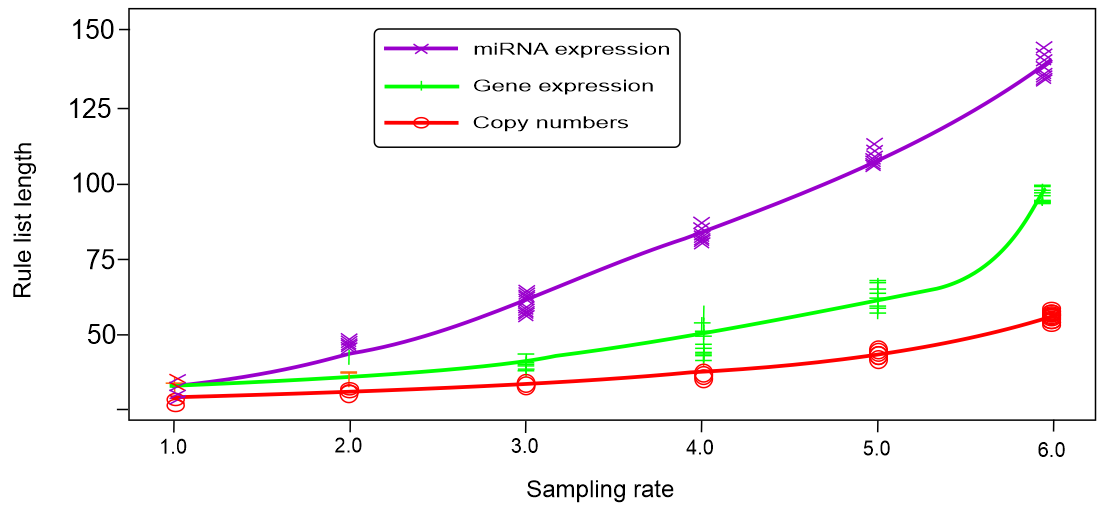
\includegraphics[width=\linewidth,height=50mm]{images/sr_vs_ll.png}
		\caption{Sampling rates vs. rule list length}
        \label{fig:lr_vs_length}
	\end{subfigure}
	\begin{subfigure}{0.48\linewidth}
		\centering
		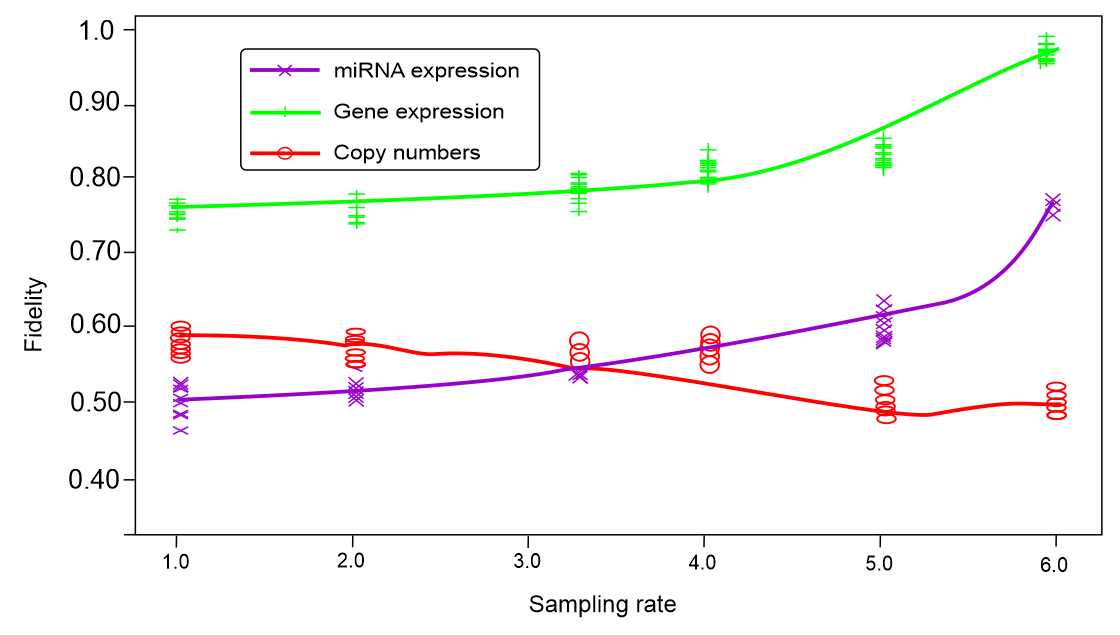
\includegraphics[width=\linewidth,height=50mm]{images/sr_vs_fide.png}
		\caption{Sampling rates vs. fidelity}
        \label{fig:lr_vs_fidelity}
	\end{subfigure}
	\caption{Effects of sampling rates on rule list length and fidelity for different single modality} 
	\label{fig:lr_vs_length_and_fidelity}
\end{figure*}

%\subsection{Effect of sampling rates on fidelity}
\hspace*{3.5mm} We study the effect of sampling rate on rule list length over three different but single modalities: gene expression, miRNA expression, and copy numbers. 
%We perform 10-fold cross-validation, such that each experiment performed 10 times to compute the fidelity on the test set. 
As shown in \cref{fig:lr_vs_fidelity}, fidelity of the extracted rule lists on all the modalities generally increases with the increased sampling rate except when the same started declining for the `copy numbers' modality when we set the sampling rate to 5.0. On the other hand, as seen we experience highest fidelities for the `gene expression' modality. In contrast,  moderately high fidelities were recorded for the 'miRNA expression' dataset, making `copy numbers' not suitable for generating and explaining diagnosis decision based on it. 

\hspace*{3.5mm} As shown in \cref{fig:lr_vs_fidelity}, with all three datasets, the fidelity of extracted rule lists generally increases as the sampling rate grows. At the same time, the complexity of the rule lists also increases drastically, exposing a trade-off between the fidelity and interpretability of the extracted rule list. Considering interpretability is our goal, we follow an intuitive strategy for choosing optimal sampling rate. We  start from a small sampling rate of 1.0, and gradually increase it until we get a good fidelity~(as shown in \cref{fig:lr_vs_fidelity}) or the length~(as shown in \cref{fig:lr_vs_length}) of the rule list exceeds an acceptable threshold. As shown in~\cref{table:rules_overall_result}, our approach generates rule lists that approximate model $f_2$ better with high fidelity on gene expression and acceptable on miRNA expression dataset. 

\subsection{Explaining the diagnoses with decision rules}
We explain both global and local behaviours of the model~($f_2$) trained on the gene expression dataset. We employ `RuleMatrix', `Skater', and `SHAP' for explaining the decisions both globally and locally. However, SHAP is used in \cref{chapter:fairness} to improve the fairness given their underlying implementation structures. A particular advantage of Skater' is that it can be used to plot the decision generated by the surrogate model in the form of decision trees. 

\subsubsection{Explaining model's global behaviour}
The data flow in \cref{fig:decision_rules_explain}, shows how all the gene expression data is captured by each of the rules. The width of the flow indicates the number of data captured and uncaptured by each rule, while the color of the flow indicates different labels. In the right of the matrix shows the fidelity and evidences. Fidelity means how accurate a rule is in approximating the $f_2$ model on the gene expression data captured by this rule. 
As stated in \cref{eq:fidelity}, fidelity ranges between 0 and 1. Hence, we plot the fidelity of the rule between 0 to 100 scale to on the subset of data satisfying the rule. As fidelity represents how accurately the rule represents the original model on this subset~\cite{ming2018rulematrix}, the higher the fidelity, the more reliable the rule is in representing the original model. The evidence or support signifies the number of data with different labels. For example, the data captured by rule 2, 3, 4, 7, 8, and 11 represent breast cancer cases. The stripped part encodes the part of data wrongly classified by the model as a certain label represent by the color.

\begin{sidewaysfigure*}
	\centering
		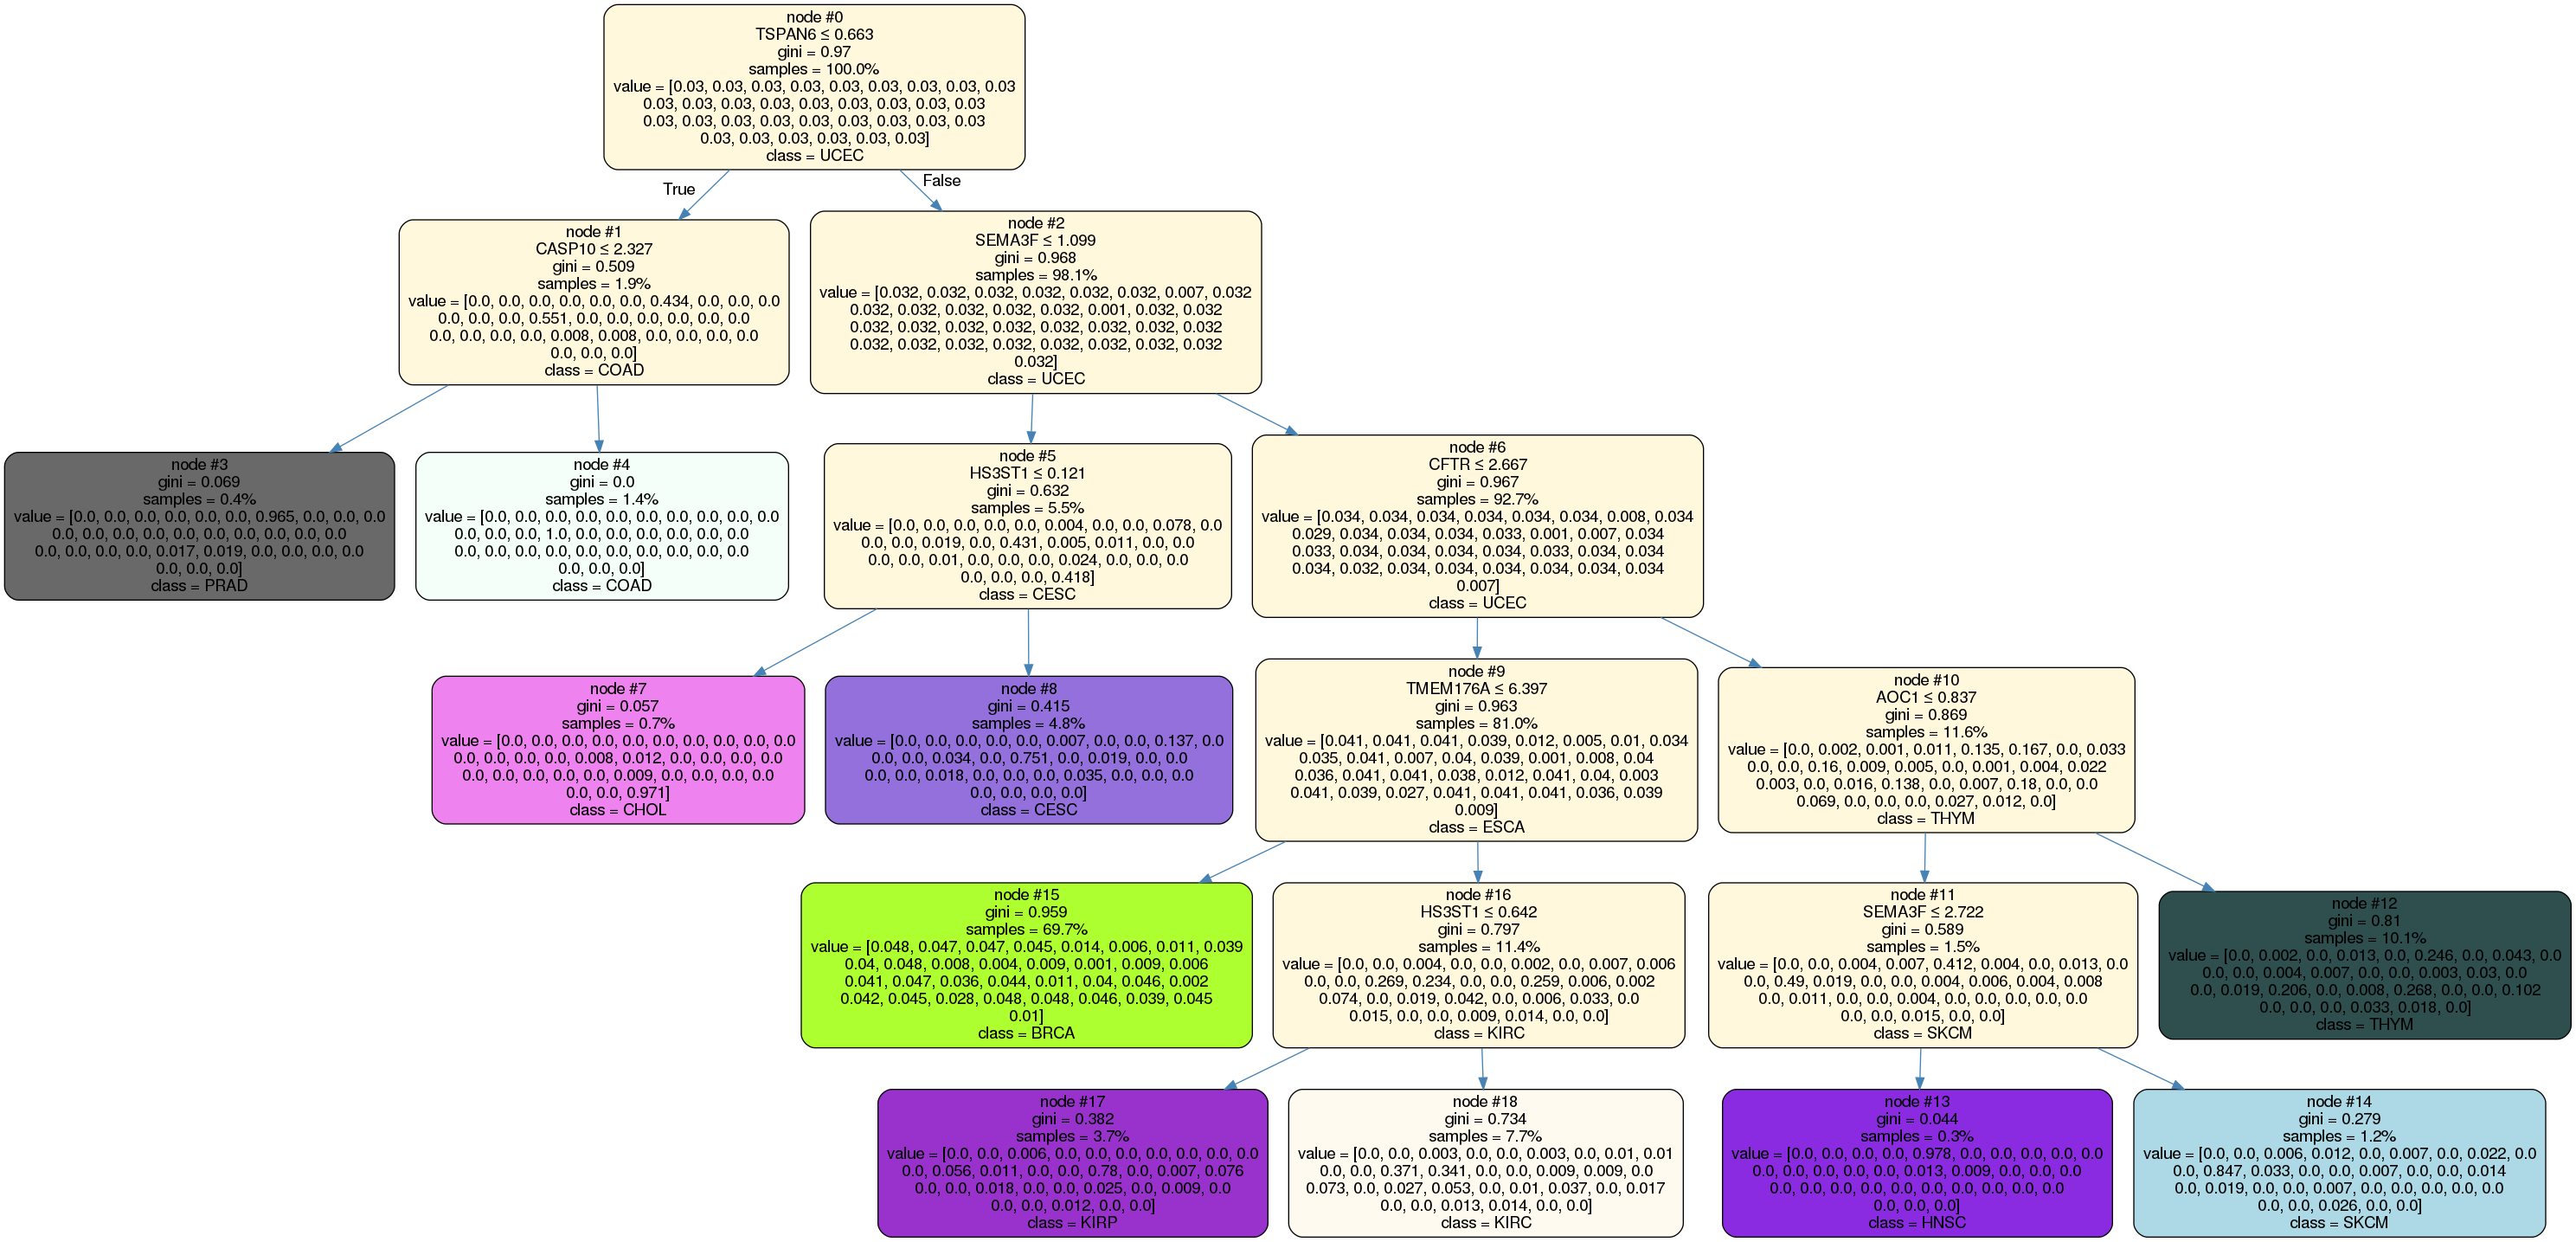
\includegraphics[scale=0.22]{images/simple_tree_pre.png}
	    \caption{Decision tree showing global decision and explanation.}
	    \label{fig:skater_global}
\end{sidewaysfigure*}

\hspace*{3.5mm} We plot the evidence w.r.t., error distribution of the model on  test set of each single modality. The horizontally stacked boxes are used to present the predictions of the model. The width of a box encodes the amount of data with a certain type of predictions. The striped boxes represent erroneous predictions, i.e., wrongly classified  sample as class blue and has true labels different from class blue. To demonstrated an example, a end user extracts a list of 10 rules from the trained model, where the default support was set to 0.1. Subsequently, he observes that rule 3 to 6 do not have enough support from the training data. Hence, he can filter the minimum evidence in the rule filter to 0.05 to collapse the last 5 rules~(rules 6 to 10). Then he finds that the first rule outputs LGG~(i.e., brain lower grade glioma) with a high probability~(i.e., 0.95) and a high fidelity~(i.e., 0.95). 

\begin{figure*}[h]
	\centering
	\captionsetup{justification=centering}
		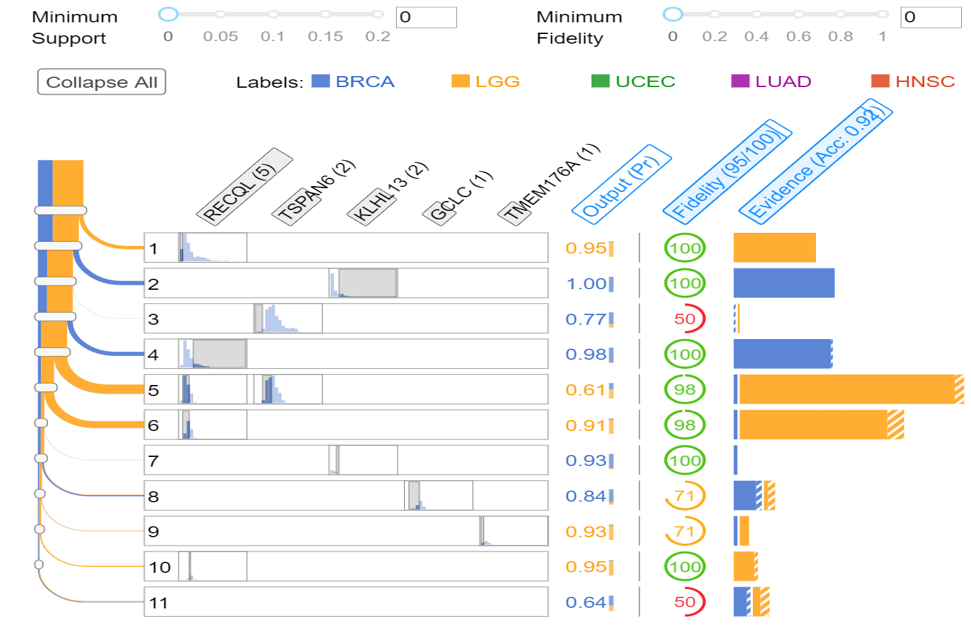
\includegraphics[scale=1.3]{images/decision_rules_explain.png}
	    \caption[Visualization of rules using rule matrix.]{The rule matrix presents each rule as a row and each feature as a column, where clauses are visualized as glyphs in the corresponding cells. The support slide-bar shows the fidelity of the rule for the sampled data, whereas the evidence signifies model's predictions and errors under a certain rule.}
	    \label{fig:decision_rules_explain}
\end{figure*}

\hspace*{3.5mm} Based on this rule matrix, he can thn learn that if the marginal adhesion score is larger than 5, the model will very likely predict brain lower grade glioma. This aligns with his knowledge that the loss of adhesion is a strong sign of cancer cells. Then he can check other rules, for example rule 2, which has the largest support from the dataset. The rule shows that if the bland chromatin is smaller or equal than 1, the cell should be kidney cancer. He then should finds this rule interesting since it indicates that one can quickly identify benign cells in the examination by checking if the nucleus is coarse. 

\begin{figure*}[h]
	\centering
		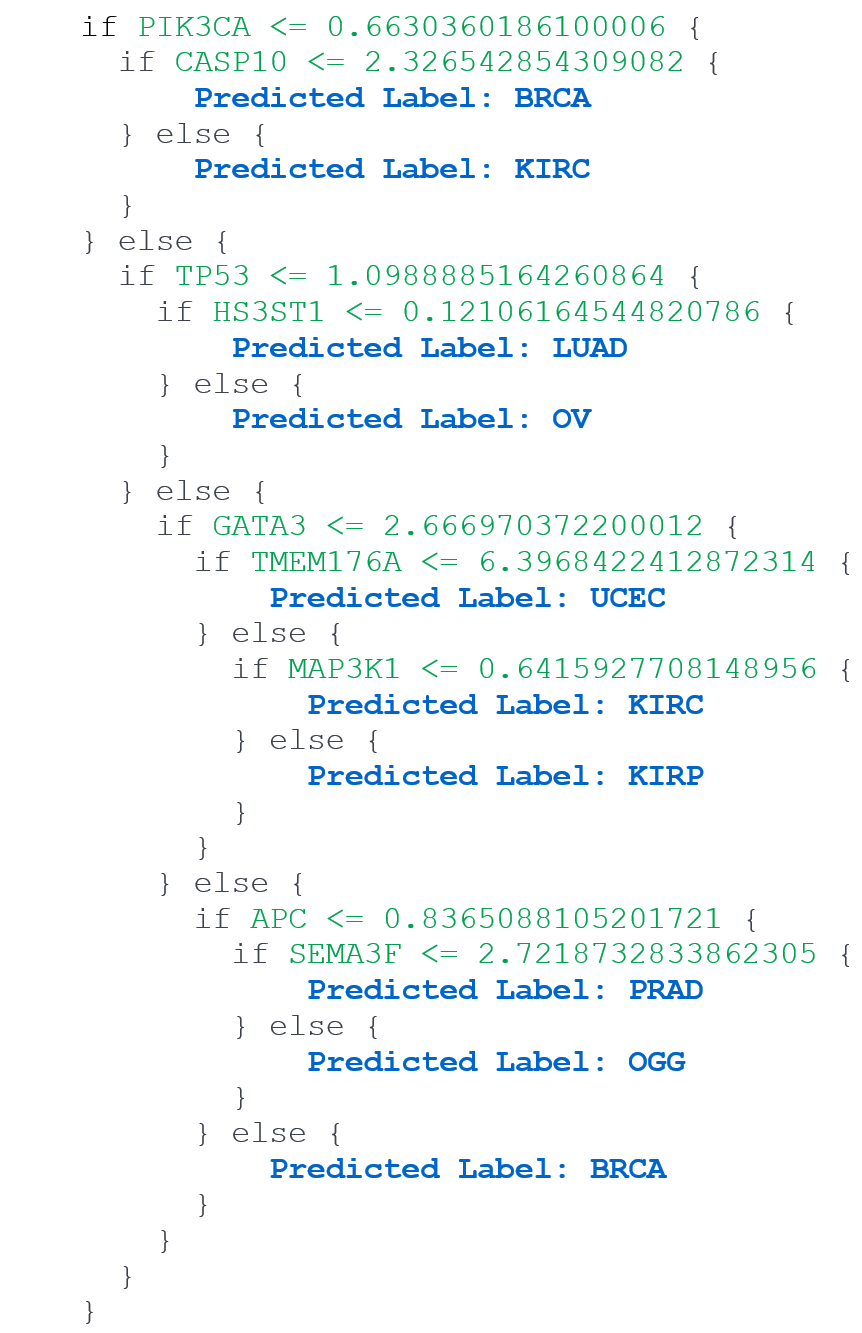
\includegraphics[scale=0.7]{images/dr_global_1.png}
	    \caption{Global decision as text based on pruned tree}
	    \label{fig:skater_decision_as_text}
	    \vspace{-2mm}
\end{figure*}

\begin{figure*}[h]
	\centering
		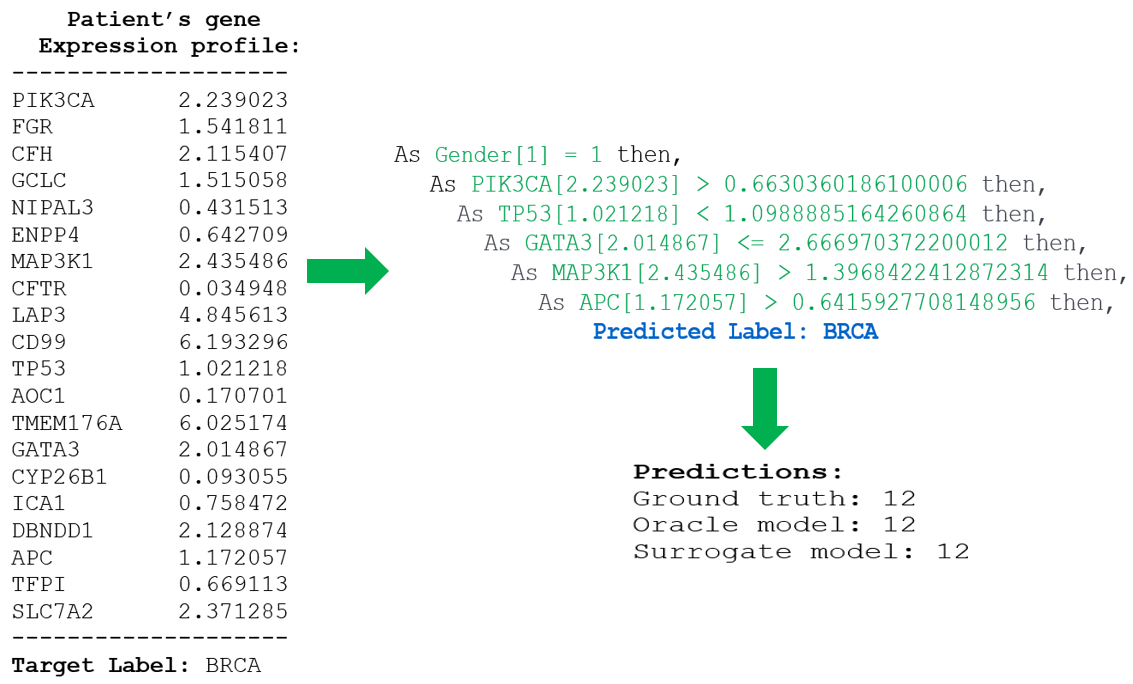
\includegraphics[scale=0.9]{images/single_pred_feature.png}
	    \caption[Local prediction for a single instance.]{Local prediction for a single instance, left: 20 features of the supplied input sample, right bottom: ground truth and the predicted labels by the oracle and the surrogate models}
	    \label{fig:decision_as_text_local_1}
\end{figure*}

\hspace*{3.5mm} \Cref{fig:skater_global} shows the global inference tree on the basis of the complete gene expression data set, where only the leaf nodes containing the respective class labels are colored~(gray, pink, purple, dark purples, green, etc.). As seen, the decision tree clearly explains how the model makes the diagnosis decision, which is already better than other charts such as feature importance and partial dependency plots, especially for the exploration and discovery. However, interpreting and explaining them to patients might be still difficult. Therefore, we use Skater to draw the global decision as text based on pruned tree in \cref{fig:skater_decision_as_text}. %The full tree for the same inferencing can be found in appendix. 

\subsubsection{Explaining model's local behaviour}
Providing human-level interpretability by ``zooming in" on individual predictions makes the explanation task easier and trustworthy\cite{ribeiro2018anchors}. When it comes to explain explaining a decision locally, we plot the decisions as text with 'Skater' by defining the scope to `local'. As seen for a single instance, both the oracle and surrogate models say that the female patient probably has breast cancer, which is based on the fact that several markers genes have contributed. 

\hspace*{3.5mm} Besides, we show how much the respective expression values for these features deviated from their base value predicted by the oracle model trained on the training set. We show the features~(only 20 features are shown for the simplicity) in the left that the mostly focused on to came up with a decision of breast cancer. We already provided the pathway enrichment analysis in \cref{chapter:xai} that also support this findings.  

\subsection{Analysis of missclassified instances}
One of the first steps towards improving an XAI system is to understand it’s weaknesses. However, weakness analysis on black-box models is not straightforward than on models which are interpretable. The better we understand what our models explain why a model works or fails in certain cases and which factors caused it to make a given prediction, the easier it becomes to improve them. Therefore, we put a close focus on the misclassified instances try to analyse the reason behind the wrong predictions. 
We further evaluate the trained model to investigate the reasons behind the incorrect predictions. The trained model~(surrogate) is being evaluated on the test set with 1,200 samples. Since, we had huge feature space, we can't confidently say the model is humanly interpretable, rather output represented as decision stumps based on significant input features, albeit we still say our model is interpretable to major extent. 

\hspace*{3.5mm} After evaluating input data at those indices, we observed that the predicted results are indeed mismatched, giving false positives or false negatives. Since, the model is interpretable, we can infer the cause of incorrect predictions with some efforts. After looking for specific misclassified instances, we found the model implies that if a patient is a male then the likelihood of his BRCA is 95\%. Since the patient in question is a male we can guess the reason behind the false positive, i.e., gender is not an important feature for male patients, while other decision rules are not contributing to the evaluation. Further, we found that both the oracle and surrogate model's predictions were the same for most of the sample examined, which is about 90\% cases, contributing about 10\% contradictory predictions. A more detailed analysis of biological signaling pathways as well as domain validation are further required to validate these findings. 

%\subsection{Discussion} \label{chapter_8:discussion}

\section{Chapter Summary} \label{chapter_7:conclusion}
In this chapter, we provide model-agnostic explanation based on IF-THEN rules for the reasoning of a model's prediction so that human users can understand. %, which will be model-agnostic explanations based on IF-THEN rules. 
Using RuleMatrix~\cite{ming2018rulematrix}, we will see how to explain individual predictions of our `black-box' models by finding a decision rule that ``anchors" the prediction sufficiently. Besides, we explain both global and local behaviours of the best model trained on the gene expression dataset. We employ `RuleMatrix', and `Skater' for explaining the decisions both globally and locally, given the fact that Skater' can be used to plot the decision generated by the surrogate model in the form of decision trees.  
%In \cref{chapter:nsr}, we will see how to combine model predictions, interpretation, and reasoning to provide more fair rules. 
Nevertheless, we analysed the limitations of our approach and missclassified instances knowing the motivations that one of the first steps towards improving an XAI system is to understand it’s weaknesses. We try to understand through a few examples why a trained model fails in certain cases and which factors caused it to make a given prediction. 

\hspace*{3.5mm} This chapter disseminates several useful findings. Based on promising results of individual metrics such as coverage, confidence, and $R^2$, it would not be unreasonable to say that we can train a surrogate model to approximate the behaviour of a complex DNN model. This also baked by the observations that both surrogate models are not only able to approximate the oracle models, but also capable of  explaining the `black-box' models. However, since $f_2$ consistently performs better in all the experiments, it would not be reasonable to replace the complex oracle models~($MCAE_{lrc}$ and $MCAE_{slr}$) with the interpretable surrogate model $f_2$. We found that decision rules are not only helpful at explaining individual diagnosis decision, but also effective at explaining both global and local behaviours of a model. Nevertheless, we explain misclassified instances using decision rules. 

\hspace*{3.5mm} An intrinsic limitation of the rule induction algorithm results from the trade-off between the fidelity and interpretability of the generated rule list. Depending on the complexity of the model and the focus of specific cancer types for which we want to make diagnostic decision, the algorithm would require a large number of rules in a rule list for the better  approximation of the model with an acceptable fidelity. The interpretability of rules also depends on the meaningfulness of the input features. Since our feature space is huge, this particularly limits the effectiveness of the model. Another reason for this is number distinct features~(apart from the huge number of genes) is low given that the feature space consists of protein-coding/oncogenes and gender. This also limits the usage of our method in other domains such as biomedical imaging, NLP, and speech recognition. Another limitation is the current unavailability of efficient learning algorithms for rule lists given the fact that we reply on the surrogate model, which is technically ensures only the representativeness, not the whole model itself. Last but not least, as we observed about 10\% contradiction between the oracle and the surrogate model's predictions this signify the surrogate model may not represent the whole behaviour of the oracle model, albeit we experienced the same prediction for 90\% of the samples examined. 

\hspace*{3.5mm} Research~\cite{POSTF} has exposed that some genes have both oncogenic and tumor-suppressor functionality. Those genes are known as proto-oncogenes with tumor-suppressor function~(POTSF). Majority of the POTSF genes act as transcription factors or kinases and exhibit dual biological functions, i.e., that they both positively and negatively regulate transcription in cells. There are some specific cancer types, e.g., leukemia are over-represented by such POTSF genes, whereas some common cancer types like lung cancer are under-represented by them~\cite{POSTF}. Therefore, in addition to the predictions, interpretations and explanation from the model, it is also important to understand and disseminate such biological instances and reason about them is important. In the next chapter, we show how the symbolic reasoning can be more effective in deducing human-understandable decision. In particular, we will answer queries posed by human operators in order to guide decision making processes in a DSS. 

